\documentclass[12pt,a4paper]{article}
\usepackage{amsmath, amssymb, geometry, booktabs, xcolor, hyperref,
            listings, pgfplots, tcolorbox, enumitem, fancyhdr, tikz, array}
\usepgfplotslibrary{fillbetween}
\geometry{margin=2.5cm}
\pgfplotsset{compat=1.18}
\tcbuselibrary{skins, breakable}

% Define custom environments
\newtcolorbox{curiositybox}[1]{colback=yellow!10, colframe=orange!80, title=#1, breakable}
\newtcolorbox{infobox}[1]{colback=blue!5, colframe=blue!60, title=#1, breakable}
\newtcolorbox{mistakebox}[1]{colback=red!5, colframe=red!60, title=#1, breakable}
\newtcolorbox{learnbox}[1]{colback=green!5, colframe=green!60, title=#1, breakable}

% Header and Footer
\pagestyle{fancy}
\fancyhf{}
\lhead{Jacobians, Functional Dependence, Taylor Expansion}
\rhead{Unit 4 -- LAC}
\cfoot{\thepage}

% Document Title Setup
\title{\textbf{Functional Dependence and Approximations} \\ \large Unit 4 -- Multivariable Differentiation and Optimization}
\author{Department of Mathematics}
\date{\today}

\begin{document}
\maketitle
\tableofcontents
\newpage

%% ============================================================
%% SECTION 1: Real-World Engineering Hook
%% ============================================================
\section{Real-World Engineering Hook}

\begin{curiositybox}{Why Should an Engineer Care?}
\textbf{Robotic Arm Singularities and the Jacobian:}
In robotic manipulators, the Jacobian matrix \( J \) maps the joint-velocity vector \( \dot{\mathbf{q}} \) to the end-effector velocity vector \( \dot{\mathbf{x}} \) via \( \dot{\mathbf{x}} = J\,\dot{\mathbf{q}} \). When the determinant of this Jacobian becomes zero, the robot hits a \emph{singular configuration}: a specific arm pose where the robot loses one or more degrees of freedom and can no longer move freely in certain directions. Engineers at Boston Dynamics and industrial automation companies must map out these singular configurations analytically before deploying a robot on an assembly line. A robot unexpectedly reaching a singularity mid-task can lock up, damage parts, or injure workers. The test \( \det(J) = 0 \) is precisely the functional-dependence criterion you will study in this unit.

\textbf{Sensor Linearization Using Taylor Expansion:}
A thermistor's resistance \( R(T) \) is a nonlinear function of temperature \( T \). Embedded systems (e.g., an ECU in an automobile engine) cannot solve the full nonlinear model in real time. Instead, the control firmware stores a second-order Taylor expansion of \( R(T) \) around a nominal operating temperature \( T_0 \):
\[
  R(T) \approx R(T_0) + R'(T_0)(T - T_0) + \tfrac{1}{2}R''(T_0)(T-T_0)^2.
\]
This polynomial approximation replaces a slow exponential computation with two multiplications and two additions, enabling $10^5$ sensor reads per second. The accuracy of the linearization---and hence the safety of the engine---depends entirely on choosing the expansion point correctly and understanding the remainder term. Both the Jacobian and Taylor expansion are therefore indispensable tools in modern engineering design.
\end{curiositybox}

%% ============================================================
%% SECTION 2: Why This Topic Exists
%% ============================================================
\section{Why This Topic Exists}

\begin{center}
\begin{tabular}{>{\bfseries}p{3.5cm} p{5cm} p{6cm}}
\toprule
Sub-Topic & Mathematical Role & Engineering Consequence \\
\midrule
Jacobians \& Functional Dependence &
  Measures how a system of functions transforms area/volume elements; detects redundant variables via \( J = 0 \). &
  Detects singular robot configurations; enables change of variables in multivariable integrals (polar, spherical); tests whether sensor equations are independent. \\[6pt]
Taylor Expansion of Two-Variable Functions &
  Provides a polynomial approximation of \( f(x,y) \) about a base point, capturing nonlinear behaviour to any desired order. &
  Linearization of coupled nonlinear ODEs in control theory; error analysis for 2D interpolation; stability analysis of equilibria in phase-plane methods. \\
\bottomrule
\end{tabular}
\end{center}

\begin{learnbox}{Core Learning Objectives}
After completing this topic you will be able to:
\begin{itemize}[leftmargin=*]
  \item Compute the Jacobian determinant of a system of two or three functions of two or three variables.
  \item Apply the functional-dependence test \( J = 0 \) to decide whether a set of functions is dependent.
  \item Perform coordinate-transform Jacobian calculations (Cartesian to polar and back).
  \item State and apply Taylor's theorem for \( f(x,y) \) to second order about any point \( (a,b) \).
  \item Write down the Maclaurin series as the special case \( (a,b) = (0,0) \).
  \item Interpret the linear approximation term as a plane tangent to the surface \( z = f(x,y) \).
\end{itemize}
\end{learnbox}

%% ============================================================
%% SECTION 3: Intuition and Definitions
%% ============================================================
\section{Intuition and Mathematical Definitions}

\subsection{Jacobians and Functional Dependence}

Imagine you have two dials, \( x \) and \( y \), that you can turn independently, and two gauges, \( u \) and \( v \), that respond to those dials. If both gauges always move together no matter which dial you turn---that is, knowing \( u \) completely determines \( v \)---then the two functions are \emph{functionally dependent}: one is essentially redundant. The Jacobian is the mathematical instrument that detects this redundancy. It measures the ``rate of area change'' when you switch from \((x,y)\)-coordinates to \((u,v)\)-coordinates; if that rate is zero everywhere, no independent 2D region maps to the output plane, and the functions are dependent.

\begin{infobox}{Jacobians and Functional Dependence --- Formal Definitions}
\textbf{Definition (2$\times$2 Jacobian).} Let \( u = u(x,y) \) and \( v = v(x,y) \) be differentiable functions. The \emph{Jacobian} of \( (u,v) \) with respect to \( (x,y) \) is:
\[
  J = \frac{\partial(u,v)}{\partial(x,y)}
    = \begin{vmatrix}
        \dfrac{\partial u}{\partial x} & \dfrac{\partial u}{\partial y} \\[8pt]
        \dfrac{\partial v}{\partial x} & \dfrac{\partial v}{\partial y}
      \end{vmatrix}
    = \frac{\partial u}{\partial x}\cdot\frac{\partial v}{\partial y}
      - \frac{\partial u}{\partial y}\cdot\frac{\partial v}{\partial x}.
\]

\textbf{Definition (3$\times$3 Jacobian).} For \( u = u(x,y,z) \), \( v = v(x,y,z) \), \( w = w(x,y,z) \):
\[
  J = \frac{\partial(u,v,w)}{\partial(x,y,z)}
    = \begin{vmatrix}
        u_x & u_y & u_z \\
        v_x & v_y & v_z \\
        w_x & w_y & w_z
      \end{vmatrix}.
\]

\textbf{Functional Dependence Test.} Functions \( u \) and \( v \) (or \( u,v,w \)) are \emph{functionally dependent} in a region \( D \) if and only if
\[
  J = \frac{\partial(u,v)}{\partial(x,y)} = 0 \quad \text{for all } (x,y) \in D.
\]
If \( J \neq 0 \) at some point, the functions are \emph{functionally independent} there.

\textbf{Coordinate Transformation (Cartesian to Polar).}
Let \( x = r\cos\theta \), \( y = r\sin\theta \). Then:
\[
  J = \frac{\partial(x,y)}{\partial(r,\theta)}
    = \begin{vmatrix}
        \cos\theta & -r\sin\theta \\
        \sin\theta &  r\cos\theta
      \end{vmatrix}
    = r\cos^{2}\!\theta + r\sin^{2}\!\theta = r.
\]
Hence \( dx\,dy = r\,dr\,d\theta \), the familiar area-element conversion in polar coordinates.

\textbf{Key Property.} If \( J_{1} = \partial(u,v)/\partial(x,y) \) and \( J_{2} = \partial(x,y)/\partial(u,v) \), then \( J_{1} \cdot J_{2} = 1 \) (reciprocal Jacobians), provided both transformations are invertible.
\end{infobox}

\noindent\textbf{Worked Example 1.1 --- Compute a Jacobian and Test Functional Dependence.}

Let \( u = x^{2} - y^{2} \) and \( v = 2xy \). Compute \( J = \partial(u,v)/\partial(x,y) \) and determine whether \( u \) and \( v \) are functionally dependent.

\textbf{Step 1: Compute partial derivatives.}
\[
  \frac{\partial u}{\partial x} = 2x, \quad
  \frac{\partial u}{\partial y} = -2y, \quad
  \frac{\partial v}{\partial x} = 2y, \quad
  \frac{\partial v}{\partial y} = 2x.
\]

\textbf{Step 2: Write and evaluate the Jacobian determinant.}
\[
  J = \begin{vmatrix} 2x & -2y \\ 2y & 2x \end{vmatrix}
    = (2x)(2x) - (-2y)(2y)
    = 4x^{2} + 4y^{2}
    = 4(x^{2} + y^{2}).
\]

\textbf{Step 3: Apply the functional-dependence test.}

\( J = 4(x^{2}+y^{2}) = 0 \) only when \( x = 0 \) and \( y = 0 \) simultaneously, i.e., only at the origin. In any region \( D \) that does not include the origin, \( J \neq 0 \), so \( u \) and \( v \) are \textbf{functionally independent}.

\textbf{Geometrical check:} note that \( u + iv = (x+iy)^{2} \), so \( u \) and \( v \) are the real and imaginary parts of a complex square. They carry independent information and cannot be expressed in terms of each other alone---confirming independence.

\subsection{Taylor Expansion of Two-Variable Functions}

For a function of one variable you learned to approximate \( f(x) \) near a point \( a \) by a polynomial. The same idea extends to two variables: we freeze a base point \( (a,b) \), let the increments be \( h = x - a \) and \( k = y - b \), and express \( f(a+h, b+k) \) as a sum of increasingly refined polynomial corrections. Each order of the expansion captures more curvature of the surface \( z = f(x,y) \), giving a better fit over a wider neighbourhood.

\begin{infobox}{Taylor's Theorem for Two-Variable Functions --- Formal Statement}
\textbf{Theorem (Taylor expansion about \( (a,b) \) to second order).}
Let \( f(x,y) \) have continuous partial derivatives up to third order in a neighbourhood of \( (a,b) \). Set \( h = x-a \), \( k = y-b \). Then:
\begin{align*}
  f(a+h, b+k) &= f(a,b) \\
  &\quad + \bigl[h\,f_{x}(a,b) + k\,f_{y}(a,b)\bigr] \\
  &\quad + \frac{1}{2!}\bigl[h^{2}\,f_{xx}(a,b) + 2hk\,f_{xy}(a,b) + k^{2}\,f_{yy}(a,b)\bigr] \\
  &\quad + R_{3},
\end{align*}
where \( R_{3} \) is the remainder (third-order and beyond).

In compact notation using the differential operator \( D = h\partial_{x} + k\partial_{y} \):
\[
  f(a+h, b+k) = \sum_{n=0}^{N} \frac{1}{n!}\,D^{n}f\Big|_{(a,b)} + R_{N+1}.
\]

\textbf{Maclaurin's Series (special case \( a = 0,\, b = 0 \)).}
\[
  f(x,y) = f(0,0) + x\,f_{x}(0,0) + y\,f_{y}(0,0)
            + \frac{1}{2}\bigl[x^{2}f_{xx}(0,0) + 2xy\,f_{xy}(0,0) + y^{2}f_{yy}(0,0)\bigr] + \cdots
\]

\textbf{Notation guide:}
\begin{itemize}[leftmargin=*]
  \item \( f_{x} = \partial f/\partial x \), \( f_{y} = \partial f/\partial y \) (first-order partials, evaluated at \( (a,b) \)).
  \item \( f_{xx} = \partial^{2}f/\partial x^{2} \), \( f_{yy} = \partial^{2}f/\partial y^{2} \), \( f_{xy} = \partial^{2}f/\partial x\partial y \) (second-order partials).
  \item By Clairaut's theorem (assuming continuity), \( f_{xy} = f_{yx} \).
\end{itemize}

\textbf{Linear approximation (first-order Taylor):}
\[
  f(x,y) \approx f(a,b) + (x-a)f_{x}(a,b) + (y-b)f_{y}(a,b).
\]
This is the equation of the tangent plane to \( z = f(x,y) \) at \( (a,b,f(a,b)) \).
\end{infobox}

\noindent\textbf{Worked Example 2.1 --- Taylor Expansion of \( f(x,y) = e^{x}\cos y \) about \( (0,0) \).}

Expand \( f(x,y) = e^{x}\cos y \) about \( (0,0) \) up to second-order terms.

\textbf{Step 1: Evaluate \( f \) at the base point.}
\[
  f(0,0) = e^{0}\cos 0 = 1\cdot 1 = 1.
\]

\textbf{Step 2: First-order partial derivatives.}
\[
  f_{x} = e^{x}\cos y \implies f_{x}(0,0) = 1.
\]
\[
  f_{y} = -e^{x}\sin y \implies f_{y}(0,0) = 0.
\]

\textbf{Step 3: Second-order partial derivatives.}
\[
  f_{xx} = e^{x}\cos y \implies f_{xx}(0,0) = 1.
\]
\[
  f_{yy} = -e^{x}\cos y \implies f_{yy}(0,0) = -1.
\]
\[
  f_{xy} = -e^{x}\sin y \implies f_{xy}(0,0) = 0.
\]

\textbf{Step 4: Assemble the Taylor expansion.}
\[
  f(x,y) \approx 1 + \bigl[x\cdot 1 + y\cdot 0\bigr]
               + \frac{1}{2}\bigl[x^{2}\cdot 1 + 2xy\cdot 0 + y^{2}\cdot(-1)\bigr]
\]
\[
  \boxed{e^{x}\cos y \approx 1 + x + \frac{x^{2} - y^{2}}{2} \quad \text{(up to second order)}.}
\]

\textbf{Engineering interpretation (sensor linearization):} Suppose a 2D sensor outputs a signal proportional to \( e^{x}\cos y \) where \( x \) and \( y \) are small deviations from nominal operating values. The linear part \( 1 + x \) gives the first-order correction to firmware calibration; the quadratic terms \( \tfrac{1}{2}(x^{2}-y^{2}) \) quantify the nonlinear crosstalk between the two channels that must be compensated in precision instrumentation. Ignoring the quadratic terms introduces a systematic error that grows as \( \sim x^{2} \) as the operating point drifts---exactly the regime modelled in thermocouple calibration tables.

%% ============================================================
%% SECTION 4: Visual Artifacts
%% ============================================================
\section{Visual Artifacts and Geometric Interpretation}

\subsection*{4.1 Cartesian-to-Polar Jacobian: Area Element Interpretation}

The following TikZ diagram shows how an infinitesimal rectangle \( dr \times d\theta \) in the polar \((r,\theta)\)-plane maps to a curved trapezoid in the Cartesian \((x,y)\)-plane. The area of that trapezoid is \( r\,dr\,d\theta \)---the Jacobian factor \( r \) arises because patches farther from the origin are physically larger.

\begin{center}
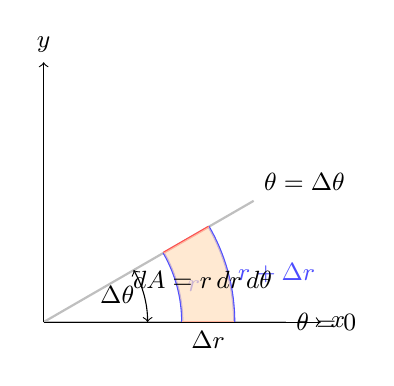
\begin{tikzpicture}[scale=2.2]
  % Draw polar grid lines (two radii)
  \draw[gray!50, thick] (0,0) -- (1.4,0) node[right, black]{\small $\theta=0$};
  \draw[gray!50, thick] (0,0) -- ({1.4*cos(30)},{1.4*sin(30)}) node[above right, black]{\small $\theta=\Delta\theta$};
  % Draw two arcs
  \draw[blue!70, thick] (0.8,0) arc (0:30:0.8) node[midway, right]{\small $r$};
  \draw[blue!70, thick] (1.1,0) arc (0:30:1.1) node[midway, right]{\small $r+\Delta r$};
  % Draw the radial sides
  \draw[red!70, thick] (0.8,0) -- (1.1,0);
  \draw[red!70, thick] ({0.8*cos(30)},{0.8*sin(30)}) -- ({1.1*cos(30)},{1.1*sin(30)});
  % Shade the area element
  \fill[orange!25, opacity=0.7]
    (0.8,0) arc(0:30:0.8) --
    ({1.1*cos(30)},{1.1*sin(30)}) arc(30:0:1.1) -- cycle;
  % Labels
  \node at ({0.95*cos(15)},{0.95*sin(15)}) {\small $dA = r\,dr\,d\theta$};
  \draw[->] (0,0) -- (0,1.5) node[above]{\small $y$};
  \draw[->] (0,0) -- (1.6,0) node[right]{\small $x$};
  \node[below] at (0.95, 0) {\small $\Delta r$};
  \draw[<->] (0.6,0) arc(0:30:0.6) node[midway, left]{\small $\Delta\theta$};
\end{tikzpicture}
\end{center}

\noindent\textit{Figure 4.1:} The shaded region is the image of the small rectangle \( [r, r+\Delta r]\times[\theta, \theta+\Delta\theta] \). Its area equals \( r\,\Delta r\,\Delta\theta \) in the limit, confirming \( J = r \) for the polar transformation.

\subsection*{4.2 Second-Order Taylor Approximation: Paraboloid Fitting a Surface}

The plot below shows the surface \( z = e^{x}\cos y \) (blue) and its second-order Taylor approximation \( z = 1 + x + \tfrac{1}{2}(x^{2}-y^{2}) \) (red) centred at the origin, illustrating how the paraboloid hugs the surface near \((0,0)\).

\begin{center}
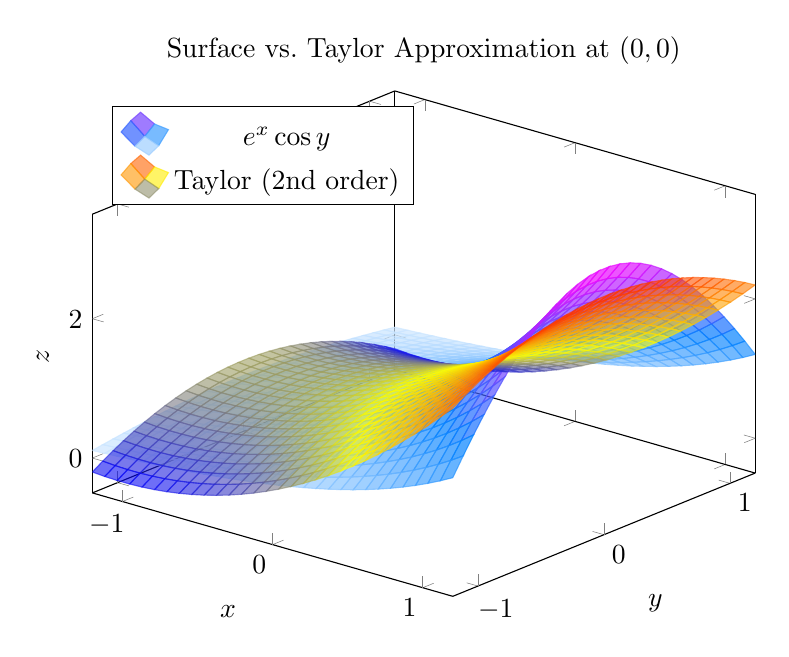
\begin{tikzpicture}
\begin{axis}[
  width=10cm, height=8cm,
  xlabel={$x$}, ylabel={$y$}, zlabel={$z$},
  title={Surface vs.\ Taylor Approximation at $(0,0)$},
  domain=-1.2:1.2, y domain=-1.2:1.2,
  samples=30,
  view={40}{30},
  colormap/cool,
  zmin=-0.5, zmax=3.5,
  legend pos=north west,
]
\addplot3[surf, opacity=0.7, shader=flat]
  {exp(x)*cos(deg(y))};
\addlegendentry{$e^{x}\cos y$}

\addplot3[surf, opacity=0.6, shader=flat, colormap/hot]
  {1 + x + 0.5*(x^2 - y^2)};
\addlegendentry{Taylor (2nd order)}
\end{axis}
\end{tikzpicture}
\end{center}

\noindent\textit{Figure 4.2:} Near the origin both surfaces nearly coincide; deviations grow as \( |(x,y)| \) increases, illustrating the local nature of Taylor approximations.

%% ============================================================
%% SECTION 5: Algorithmic Workflow
%% ============================================================
\section{Step-by-Step Algorithmic Workflow}

\begin{infobox}{Algorithm A --- Computing a 2$\times$2 Jacobian}
\begin{enumerate}[leftmargin=*, label=\textbf{Step \arabic*.}]
  \item Write down the two functions \( u(x,y) \) and \( v(x,y) \).
  \item Compute all four first-order partial derivatives: \( u_x,\, u_y,\, v_x,\, v_y \).
  \item Form the determinant:
    \[
      J = \begin{vmatrix} u_x & u_y \\ v_x & v_y \end{vmatrix} = u_x v_y - u_y v_x.
    \]
  \item Simplify the expression for \( J \).
\end{enumerate}
\end{infobox}

\begin{infobox}{Algorithm B --- Testing Functional Dependence}
\begin{enumerate}[leftmargin=*, label=\textbf{Step \arabic*.}]
  \item Compute \( J = \partial(u,v)/\partial(x,y) \) using Algorithm A.
  \item If \( J = 0 \) identically (for all \( x,y \) in the domain), conclude \textbf{functionally dependent}.
  \item If \( J \neq 0 \) at even one point of the domain, conclude \textbf{functionally independent} in that region.
  \item (Optional verification) Try to eliminate \( x \) and \( y \) to express \( v \) as a function of \( u \) alone. If successful, the functions are dependent.
\end{enumerate}
\end{infobox}

\begin{infobox}{Algorithm C --- Constructing a 2-Variable Taylor Expansion to Degree 2}
\begin{enumerate}[leftmargin=*, label=\textbf{Step \arabic*.}]
  \item Identify the base point \( (a,b) \) and set \( h = x - a \), \( k = y - b \).
  \item Evaluate \( f(a,b) \).
  \item Compute and evaluate the first-order partials: \( f_x(a,b) \) and \( f_y(a,b) \).
  \item Compute and evaluate the three second-order partials: \( f_{xx}(a,b) \), \( f_{xy}(a,b) \), \( f_{yy}(a,b) \).
  \item Assemble:
    \[
      f(x,y) \approx f(a,b) + hf_x + kf_y + \tfrac{1}{2}(h^2 f_{xx} + 2hk\,f_{xy} + k^2 f_{yy}).
    \]
  \item Substitute \( h = x-a \) and \( k = y-b \) back to express the result in \( x \) and \( y \).
\end{enumerate}
\end{infobox}

%% ============================================================
%% SECTION 6: Fully Worked Numerical Examples
%% ============================================================
\section{Fully Worked Step-by-Step Numerical Examples}

\subsection*{Example 1 --- Jacobian of \( u = x^{2}-y^{2},\; v = 2xy \)}

\textbf{Given:} \( u = x^{2} - y^{2} \), \( v = 2xy \).

Compute \( J = \partial(u,v)/\partial(x,y) \) and test functional dependence.

\textbf{Partial derivatives:}
\[
  u_x = 2x,\quad u_y = -2y,\quad v_x = 2y,\quad v_y = 2x.
\]

\textbf{Jacobian:}
\[
  J = \begin{vmatrix} 2x & -2y \\ 2y & 2x \end{vmatrix}
    = (2x)(2x) - (-2y)(2y)
    = 4x^{2} + 4y^{2}
    = 4(x^{2}+y^{2}).
\]

\textbf{Conclusion:} \( J = 4(x^{2}+y^{2}) \neq 0 \) for \( (x,y) \neq (0,0) \), so \( u \) and \( v \) are \textbf{functionally independent} everywhere except the origin.

\textbf{Algebraic check:} From \( u = x^{2}-y^{2} \) and \( v = 2xy \), we get \( u^{2}+v^{2} = (x^{2}-y^{2})^{2} + 4x^{2}y^{2} = (x^{2}+y^{2})^{2} \). This is a relation involving both \( u \) and \( v \) as well as \( x^{2}+y^{2} \), so \( v \) cannot be written as a function of \( u \) alone --- confirming independence.

\subsection*{Example 2 --- Polar Transformation Jacobian}

\textbf{Given:} \( x = r\cos\theta \), \( y = r\sin\theta \). Compute \( J = \partial(x,y)/\partial(r,\theta) \) and verify \( J = r \).

\textbf{Partial derivatives:}
\[
  \frac{\partial x}{\partial r} = \cos\theta, \quad
  \frac{\partial x}{\partial \theta} = -r\sin\theta, \quad
  \frac{\partial y}{\partial r} = \sin\theta, \quad
  \frac{\partial y}{\partial \theta} = r\cos\theta.
\]

\textbf{Jacobian determinant:}
\[
  J = \begin{vmatrix}
    \cos\theta & -r\sin\theta \\
    \sin\theta &  r\cos\theta
  \end{vmatrix}
  = \cos\theta \cdot r\cos\theta - (-r\sin\theta)\cdot\sin\theta.
\]
\[
  = r\cos^{2}\theta + r\sin^{2}\theta = r(\cos^{2}\theta + \sin^{2}\theta) = r.
\]

\textbf{Conclusion:} \( J = r \geq 0 \). The area element transforms as \( dx\,dy = r\,dr\,d\theta \). For \( r > 0 \) the transformation is invertible; at \( r = 0 \) (the origin) \( J = 0 \) and the transformation degenerates (the entire circle of radius 0 maps to a single point).

\subsection*{Example 3 --- Taylor Expansion: \( f(x,y) = e^{x}\cos y \) about \( (0,0) \)}

Expand \( f(x,y) = e^{x}\cos y \) about \( (0,0) \) up to second-order terms and interpret physically.

\textbf{Step 1: Base point value.}
\[
  f(0,0) = e^{0}\cos 0 = 1.
\]

\textbf{Step 2: First-order partials.}
\[
  f_x = e^{x}\cos y \implies f_x(0,0) = 1.
\]
\[
  f_y = -e^{x}\sin y \implies f_y(0,0) = 0.
\]

\textbf{Step 3: Second-order partials.}
\[
  f_{xx} = e^{x}\cos y \implies f_{xx}(0,0) = 1.
\]
\[
  f_{yy} = -e^{x}\cos y \implies f_{yy}(0,0) = -1.
\]
\[
  f_{xy} = -e^{x}\sin y \implies f_{xy}(0,0) = 0.
\]

\textbf{Step 4: Assemble Maclaurin expansion.}
\[
  e^{x}\cos y \approx 1 + (1\cdot x + 0\cdot y) + \frac{1}{2}(1\cdot x^{2} + 2\cdot 0 \cdot xy + (-1)\cdot y^{2})
\]
\[
  \boxed{e^{x}\cos y \approx 1 + x + \frac{x^{2}-y^{2}}{2}.}
\]

\textbf{Engineering interpretation:} In a 2D sensor array, suppose channel outputs are \( S_{1} = e^{x}\cos y \) where \( x, y \) are small thermal drift variables. The zeroth-order term \( 1 \) is the nominal output. The linear term \( x \) captures the dominant drift contribution from the first channel. The quadratic cross-term \( -y^{2}/2 \) reveals that drift in the second channel always \emph{reduces} the output (negative curvature in \( y \)), so over-temperature in channel 2 causes systematic underestimation of the true signal---a bias that must be corrected in calibration firmware.

%% ============================================================
%% SECTION 7: Tabular Reference
%% ============================================================
\section{Tabular Comparison: 1-Variable vs.\ 2-Variable Taylor Series}

\begin{center}
\begin{tabular}{>{\bfseries}p{3.2cm} p{5cm} p{5.5cm}}
\toprule
Feature & 1-Variable Taylor Series & 2-Variable Taylor Series \\
\midrule
General formula &
  \( f(a+h) = \displaystyle\sum_{n=0}^{N}\frac{h^n}{n!}f^{(n)}(a) + R_N \) &
  \( f(a+h,b+k) = \displaystyle\sum_{n=0}^{N}\frac{1}{n!}(h\partial_x+k\partial_y)^n f\big|_{(a,b)} + R_N \) \\[8pt]
Second-order terms &
  \( f(a) + hf'(a) + \tfrac{h^2}{2}f''(a) \) &
  \( f + hf_x + kf_y + \tfrac{1}{2}(h^2f_{xx}+2hkf_{xy}+k^2f_{yy}) \) \\[8pt]
Maclaurin form &
  Expand about \( a = 0 \) &
  Expand about \( (a,b)=(0,0) \) \\[8pt]
Convergence &
  Radius of convergence \( R \): series valid for \( |h| < R \) &
  Region of convergence is a disk \( \sqrt{h^2+k^2} < R \) in 2D \\[8pt]
Geometric meaning &
  Tangent line approximation at 1st order &
  Tangent plane approximation at 1st order; paraboloid at 2nd order \\[8pt]
Number of nth-order terms &
  1 term of each order &
  \( n+1 \) distinct terms of order \( n \) (mixed partials) \\[8pt]
Engineering use &
  ODE linearization, root finding (Newton--Raphson), 1D sensor calibration &
  2D sensor linearization, Jacobian-based control, stability analysis of 2D equilibria \\
\bottomrule
\end{tabular}
\end{center}

%% ============================================================
%% SECTION 8: Common Mistakes
%% ============================================================
\section{Common Student Mistakes and Pitfalls}

\begin{mistakebox}{Common Mistakes --- Jacobians and Taylor Expansions}
\begin{tabular}{>{\bfseries}p{3.8cm} p{5cm} p{5cm}}
\toprule
Mistake & Why It Goes Wrong & Correct Approach \\
\midrule
Wrong row order in Jacobian &
  Writing \( \partial(x,y)/\partial(u,v) \) when the problem asks for \( \partial(u,v)/\partial(x,y) \), giving the reciprocal determinant. &
  Always put the ``output'' variables in the numerator and the ``input'' variables in the denominator; rows correspond to the numerator functions. \\[6pt]
Concluding dependence from \( J=0 \) at one point only &
  \( J = 4(x^{2}+y^{2}) = 0 \) only at the origin; declaring the functions dependent everywhere. &
  Functional dependence requires \( J = 0 \) \emph{identically} on the entire domain, not just at isolated points. \\[6pt]
Missing the factor 2 on the mixed partial &
  Writing \( \tfrac{1}{2}(h^2 f_{xx} + hk\,f_{xy} + k^2 f_{yy}) \) instead of the correct \( 2hk\,f_{xy} \). &
  The cross-term coefficient is \( 2hk\,f_{xy} \) because \( f_{xy} = f_{yx} \) and both appear when expanding \( (h\partial_x+k\partial_y)^2 \). \\[6pt]
Evaluating partials at \( (x,y) \) not at \( (a,b) \) &
  Leaving \( f_{xx} = e^{x}\cos y \) without substituting \( (0,0) \), then using the un-evaluated expression in the expansion. &
  Always evaluate all partial derivatives at the expansion point \emph{before} writing the Taylor polynomial. \\[6pt]
Forgetting that \( J = r \) is always non-negative &
  Stating the polar Jacobian as \( \pm r \) or treating \( r \) as possibly negative. &
  By convention \( r \geq 0 \) in polar coordinates, so \( J = r \geq 0 \) and area elements are always positive. \\[6pt]
Incorrect determinant expansion (sign error) &
  Computing \( \begin{vmatrix} a & b \\ c & d \end{vmatrix} = ad + bc \) instead of \( ad - bc \). &
  Determinant of a \( 2\times 2 \) matrix is \emph{always} \( ad - bc \) (subtract the off-diagonal product). \\
\bottomrule
\end{tabular}
\end{mistakebox}

%% ============================================================
%% SECTION 9: Assessment Suite
%% ============================================================
\section{Comprehensive Assessment Suite}

\subsection*{9.1 Viva-Voce Questions}

\begin{enumerate}[leftmargin=*, label=\textbf{Q\arabic*.}]

  \item \textbf{[Sub-topic 1]} Define the Jacobian \( \partial(u,v)/\partial(x,y) \). What does it geometrically represent in the context of coordinate transformations?

  \textit{Expected answer:} The Jacobian is the determinant of the matrix of first-order partial derivatives of \( (u,v) \) with respect to \( (x,y) \). Geometrically it represents the ratio of an infinitesimal area element in the \( (u,v) \)-plane to the corresponding area element in the \( (x,y) \)-plane under the transformation.

  \item \textbf{[Sub-topic 1]} State the functional-dependence test. Give one example of functionally dependent functions.

  \textit{Expected answer:} Functions \( u(x,y) \) and \( v(x,y) \) are functionally dependent if and only if their Jacobian \( \partial(u,v)/\partial(x,y) = 0 \) identically. Example: \( u = x+y \), \( v = (x+y)^{2} \) are dependent because \( v = u^{2} \).

  \item \textbf{[Sub-topic 1]} Verify that the Jacobian of the polar transformation is \( r \). Why does this imply \( dx\,dy = r\,dr\,d\theta \)?

  \textit{Expected answer:} Compute \( \partial(x,y)/\partial(r,\theta) \) for \( x = r\cos\theta \), \( y = r\sin\theta \): the determinant equals \( r\cos^2\theta + r\sin^2\theta = r \). The change-of-variables formula for multiple integrals states that the area element transforms as \( dx\,dy = |J|\,dr\,d\theta \), so \( dx\,dy = r\,dr\,d\theta \) (with \( r \geq 0 \)).

  \item \textbf{[Sub-topic 1]} If \( J_1 = \partial(u,v)/\partial(x,y) \) and \( J_2 = \partial(x,y)/\partial(u,v) \), what is their product?

  \textit{Expected answer:} \( J_1 \cdot J_2 = 1 \), provided the transformation is invertible. This is analogous to the chain rule for ordinary derivatives: \( (dy/dx)\cdot(dx/dy) = 1 \).

  \item \textbf{[Sub-topic 2]} State Taylor's theorem for a function of two variables \( f(x,y) \) about the point \( (a,b) \) up to second-order terms. Identify each term.

  \textit{Expected answer:} \( f(a+h,b+k) = f(a,b) + hf_x + kf_y + \tfrac{1}{2}(h^2f_{xx}+2hkf_{xy}+k^2f_{yy}) + \ldots \), where \( h=x-a \), \( k=y-b \), and all partials are evaluated at \( (a,b) \). The first line is the value, the second is the linear (tangent-plane) correction, the third is the quadratic (paraboloid) correction.

  \item \textbf{[Sub-topic 2]} What is Maclaurin's series? How does it relate to Taylor's series?

  \textit{Expected answer:} Maclaurin's series is the Taylor series with the expansion point at the origin: \( (a,b) = (0,0) \). It is a special case of Taylor's series, useful when the function has a simple form near the origin.

  \item \textbf{[Sub-topic 2]} What is the geometric meaning of the first-order Taylor approximation of \( f(x,y) \)?

  \textit{Expected answer:} The first-order approximation \( f(a,b) + (x-a)f_x(a,b) + (y-b)f_y(a,b) \) is the equation of the \emph{tangent plane} to the surface \( z = f(x,y) \) at the point \( (a,b,f(a,b)) \).

  \item \textbf{[Sub-topic 2]} For \( f(x,y) = \sin x \cos y \), what is the linear approximation about \( (0,0) \)?

  \textit{Expected answer:} \( f_x = \cos x\cos y \implies f_x(0,0) = 1 \); \( f_y = -\sin x\sin y \implies f_y(0,0) = 0 \); \( f(0,0) = 0 \). So the linear approximation is \( f(x,y) \approx x \).

\end{enumerate}

\subsection*{9.2 Descriptive Exam Questions}

\begin{enumerate}[leftmargin=*, label=\textbf{D\arabic*.}]

  \item \textbf{[Sub-topic 1]} If \( u = x^{2} + y^{2} \) and \( v = 2\arctan(y/x) \), find the Jacobian \( \partial(u,v)/\partial(x,y) \). Are \( u \) and \( v \) functionally dependent?

  \textit{Hint:} Compute \( u_x = 2x \), \( u_y = 2y \), \( v_x = -2y/(x^2+y^2) \), \( v_y = 2x/(x^2+y^2) \). Form the determinant and simplify. Note that \( u = r^{2} \) and \( v = 2\theta \) in polar coordinates, so they carry independent information about \( r \) and \( \theta \) separately --- check by computing \( J \) and verifying it is non-zero.

  \item \textbf{[Sub-topic 1]} For the 3D transformation \( u = x+y+z \), \( v = xy+yz+zx \), \( w = xyz \), write the \( 3\times 3 \) Jacobian matrix and describe (without necessarily expanding the full determinant) why these three elementary symmetric functions might be expected to be functionally independent for generic \( (x,y,z) \).

  \textit{Hint:} Set up the \( 3\times 3 \) matrix. Note that \( u, v, w \) are the elementary symmetric polynomials whose independence is tied to the invertibility of the Vandermonde-type structure.

  \item \textbf{[Sub-topic 2]} Expand \( f(x,y) = \ln(1+x+y) \) about \( (0,0) \) up to second-order terms in \( x \) and \( y \). Hence find an approximate value of \( \ln(1.1 + 0.2) \).

  \textit{Hint:} \( f(0,0)=0 \); \( f_x = f_y = 1/(1+x+y) \) so \( f_x(0,0) = f_y(0,0) = 1 \); \( f_{xx} = f_{yy} = f_{xy} = -1/(1+x+y)^{2} \) so all second partials equal \( -1 \) at origin. Expansion: \( (x+y) - \tfrac{1}{2}(x+y)^{2} + \ldots \) Substitute \( x=0.1, y=0.2 \).

  \item \textbf{[Sub-topic 2]} Find the Taylor expansion of \( f(x,y) = e^{xy} \) about \( (1,1) \) up to second-order terms.

  \textit{Hint:} Set \( h = x-1 \), \( k = y-1 \). Compute: \( f(1,1) = e \); \( f_x = ye^{xy} \implies f_x(1,1) = e \); \( f_y = xe^{xy} \implies f_y(1,1) = e \); \( f_{xx} = y^2 e^{xy} \implies e \); \( f_{yy} = x^2 e^{xy} \implies e \); \( f_{xy} = (1+xy)e^{xy} \implies 2e \). Assemble.

  \item \textbf{[Sub-topics 1 \& 2]} In a robotic wrist joint, the end-effector position is given by \( x = L_1\cos\theta_1 + L_2\cos(\theta_1+\theta_2) \) and \( y = L_1\sin\theta_1 + L_2\sin(\theta_1+\theta_2) \). Derive the \( 2\times 2 \) Jacobian \( \partial(x,y)/\partial(\theta_1,\theta_2) \) and find the condition on \( \theta_2 \) for a singular configuration (\( J = 0 \)).

  \textit{Hint:} After differentiating, the Jacobian determinant simplifies to \( L_1 L_2 \sin\theta_2 \). Singularity occurs when \( \theta_2 = 0 \) or \( \theta_2 = \pi \) (arm fully extended or fully folded).

\end{enumerate}

\subsection*{9.3 Multiple Choice Questions}

\begin{enumerate}[leftmargin=*, label=\textbf{MCQ\arabic*.}]

  \item \textbf{[Sub-topic 1]} If \( u = x^{2}-y^{2} \) and \( v = 2xy \), the Jacobian \( \partial(u,v)/\partial(x,y) \) equals:
  \begin{enumerate}[label=(\Alph*)]
    \item \( 4xy \)
    \item \( 4(x-y)(x+y) \)
    \item \textbf{\( 4(x^{2}+y^{2}) \)}
    \item \( 2(x^{2}-y^{2}) \)
  \end{enumerate}
  \textit{Explanation:} \( J = (2x)(2x)-(-2y)(2y) = 4x^2+4y^2 = 4(x^2+y^2) \).

  \item \textbf{[Sub-topic 1]} The Jacobian of the polar transformation \( x = r\cos\theta,\; y = r\sin\theta \) is:
  \begin{enumerate}[label=(\Alph*)]
    \item \( 1 \)
    \item \( r^{2} \)
    \item \textbf{\( r \)}
    \item \( \cos\theta + \sin\theta \)
  \end{enumerate}
  \textit{Explanation:} The determinant \( \cos\theta\cdot r\cos\theta - (-r\sin\theta)\cdot\sin\theta = r(\cos^2\theta+\sin^2\theta) = r \).

  \item \textbf{[Sub-topic 1]} Functions \( u \) and \( v \) are functionally dependent if:
  \begin{enumerate}[label=(\Alph*)]
    \item \( \partial(u,v)/\partial(x,y) \neq 0 \) everywhere
    \item \( \partial(u,v)/\partial(x,y) = 0 \) at one isolated point
    \item \textbf{\( \partial(u,v)/\partial(x,y) = 0 \) identically over the domain}
    \item \( u = v \) at every point
  \end{enumerate}
  \textit{Explanation:} Functional dependence requires the Jacobian to vanish throughout the domain, not merely at an isolated point.

  \item \textbf{[Sub-topic 2]} The second-order Taylor expansion of \( f(x,y) = e^{x}\cos y \) about \( (0,0) \) is:
  \begin{enumerate}[label=(\Alph*)]
    \item \( 1 + x + y + \tfrac{1}{2}(x^{2}+y^{2}) \)
    \item \( 1 + x - y + \tfrac{1}{2}(x^{2}-y^{2}) \)
    \item \textbf{\( 1 + x + \tfrac{1}{2}(x^{2}-y^{2}) \)}
    \item \( x + \tfrac{1}{2}x^{2} - \tfrac{1}{2}y^{2} \)
  \end{enumerate}
  \textit{Explanation:} \( f_y(0,0) = 0 \) (since \( f_y = -e^x\sin y \) and \( \sin 0 = 0 \)), so the \( y \) linear term vanishes; \( f_{yy}(0,0) = -1 \) gives the \( -y^{2}/2 \) term.

  \item \textbf{[Sub-topic 2]} Maclaurin's series for \( f(x,y) \) is the Taylor series expanded about:
  \begin{enumerate}[label=(\Alph*)]
    \item \( (1,0) \)
    \item \( (a,b) \) for arbitrary \( (a,b) \)
    \item \textbf{\( (0,0) \)}
    \item \( (\infty,\infty) \)
  \end{enumerate}
  \textit{Explanation:} Maclaurin's series is the special case of Taylor's theorem at the origin \( (a,b)=(0,0) \).

  \item \textbf{[Sub-topic 2]} The first-order Taylor approximation of \( f(x,y) \) at \( (a,b) \) represents geometrically:
  \begin{enumerate}[label=(\Alph*)]
    \item A sphere centred at \( (a,b,f(a,b)) \)
    \item The osculating paraboloid at \( (a,b) \)
    \item \textbf{The tangent plane to the surface \( z = f(x,y) \) at \( (a,b,f(a,b)) \)}
    \item A horizontal plane at height \( f(a,b) \)
  \end{enumerate}
  \textit{Explanation:} The linear approximation \( f(a,b)+(x-a)f_x+(y-b)f_y \) is exactly the equation of the tangent plane, with gradient vector \( (f_x, f_y) \) as the slope in each direction.

\end{enumerate}

%% ============================================================
%% SECTION 10: Quick Recap and Formula Sheet
%% ============================================================
\section{Quick Recap and Formula Sheet}

\begin{learnbox}{Formula Sheet --- Jacobians and Taylor Expansion}
\begin{itemize}[leftmargin=*]
  \item \textbf{2$\times$2 Jacobian determinant:}
    \( J = \dfrac{\partial(u,v)}{\partial(x,y)} =
    \begin{vmatrix} u_x & u_y \\ v_x & v_y \end{vmatrix}
    = u_x v_y - u_y v_x. \)
  \item \textbf{Functional dependence test:} \( u \) and \( v \) are functionally dependent \( \iff J = 0 \) identically on the domain; if \( J \neq 0 \) at any point, they are independent there.
  \item \textbf{Polar Jacobian:} \( \dfrac{\partial(x,y)}{\partial(r,\theta)} = r \); hence the area element \( dx\,dy = r\,dr\,d\theta \).
  \item \textbf{2-variable Taylor series (about \( (a,b) \), up to 2nd order):}
    \[
      f(a+h,b+k) \approx f(a,b) + hf_x + kf_y + \tfrac{1}{2}(h^2 f_{xx} + 2hkf_{xy} + k^2 f_{yy}),
    \]
    where \( h = x-a \), \( k = y-b \), and partials evaluated at \( (a,b) \).
  \item \textbf{Maclaurin form (\( (a,b) = (0,0) \)):}
    \( f(x,y) \approx f_{00} + xf_x + yf_y + \tfrac{1}{2}(x^2 f_{xx}+2xyf_{xy}+y^2 f_{yy}) \).
  \item \textbf{Reciprocal Jacobian property:}
    \( \dfrac{\partial(u,v)}{\partial(x,y)} \cdot \dfrac{\partial(x,y)}{\partial(u,v)} = 1 \) (invertible transformations).
  \item \textbf{Linear (1st-order) approximation = tangent plane:}
    \( f(x,y) \approx f(a,b) + (x-a)f_x(a,b) + (y-b)f_y(a,b). \)
  \item \textbf{Mixed-partial symmetry:} By Clairaut's theorem, \( f_{xy} = f_{yx} \) when both are continuous, so the cross-term in the quadratic form is \( 2hkf_{xy} \) (factor of 2, not 1).
\end{itemize}
\end{learnbox}

\end{document}
